%%
% Copyright (c) 2017 - 2020, Pascal Wagler;
% Copyright (c) 2014 - 2020, John MacFarlane
%
% All rights reserved.
%
% Redistribution and use in source and binary forms, with or without
% modification, are permitted provided that the following conditions
% are met:
%
% - Redistributions of source code must retain the above copyright
% notice, this list of conditions and the following disclaimer.
%
% - Redistributions in binary form must reproduce the above copyright
% notice, this list of conditions and the following disclaimer in the
% documentation and/or other materials provided with the distribution.
%
% - Neither the name of John MacFarlane nor the names of other
% contributors may be used to endorse or promote products derived
% from this software without specific prior written permission.
%
% THIS SOFTWARE IS PROVIDED BY THE COPYRIGHT HOLDERS AND CONTRIBUTORS
% "AS IS" AND ANY EXPRESS OR IMPLIED WARRANTIES, INCLUDING, BUT NOT
% LIMITED TO, THE IMPLIED WARRANTIES OF MERCHANTABILITY AND FITNESS
% FOR A PARTICULAR PURPOSE ARE DISCLAIMED. IN NO EVENT SHALL THE
% COPYRIGHT OWNER OR CONTRIBUTORS BE LIABLE FOR ANY DIRECT, INDIRECT,
% INCIDENTAL, SPECIAL, EXEMPLARY, OR CONSEQUENTIAL DAMAGES (INCLUDING,
% BUT NOT LIMITED TO, PROCUREMENT OF SUBSTITUTE GOODS OR SERVICES;
% LOSS OF USE, DATA, OR PROFITS; OR BUSINESS INTERRUPTION) HOWEVER
% CAUSED AND ON ANY THEORY OF LIABILITY, WHETHER IN CONTRACT, STRICT
% LIABILITY, OR TORT (INCLUDING NEGLIGENCE OR OTHERWISE) ARISING IN
% ANY WAY OUT OF THE USE OF THIS SOFTWARE, EVEN IF ADVISED OF THE
% POSSIBILITY OF SUCH DAMAGE.
%%

%%
% This is the Eisvogel pandoc LaTeX template.
%
% For usage information and examples visit the official GitHub page:
% https://github.com/Wandmalfarbe/pandoc-latex-template
%%



% Options for packages loaded elsewhere
\PassOptionsToPackage{unicode}{hyperref}
\PassOptionsToPackage{hyphens}{url}
\PassOptionsToPackage{dvipsnames,svgnames*,x11names*,table}{xcolor}
%
\documentclass[
  paper=a4,
,captions=tableheading
]{scrartcl}
\usepackage{lmodern}
\usepackage{setspace}
\setstretch{1.2}
\usepackage{amssymb,amsmath}
\usepackage{ifxetex,ifluatex}
\ifnum 0\ifxetex 1\fi\ifluatex 1\fi=0 % if pdftex
  \usepackage[T1]{fontenc}
  \usepackage[utf8]{inputenc}
  \usepackage{textcomp} % provide euro and other symbols
\else % if luatex or xetex
  \usepackage{unicode-math}
  \defaultfontfeatures{Scale=MatchLowercase}
  \defaultfontfeatures[\rmfamily]{Ligatures=TeX,Scale=1}
\fi
% Use upquote if available, for straight quotes in verbatim environments
\IfFileExists{upquote.sty}{\usepackage{upquote}}{}
\IfFileExists{microtype.sty}{% use microtype if available
  \usepackage[]{microtype}
  \UseMicrotypeSet[protrusion]{basicmath} % disable protrusion for tt fonts
}{}
\makeatletter
\@ifundefined{KOMAClassName}{% if non-KOMA class
  \IfFileExists{parskip.sty}{%
    \usepackage{parskip}
  }{% else
    \setlength{\parindent}{0pt}
    \setlength{\parskip}{6pt plus 2pt minus 1pt}}
}{% if KOMA class
  \KOMAoptions{parskip=half}}
\makeatother
\usepackage{xcolor}
\definecolor{default-linkcolor}{HTML}{A50000}
\definecolor{default-filecolor}{HTML}{A50000}
\definecolor{default-citecolor}{HTML}{4077C0}
\definecolor{default-urlcolor}{HTML}{4077C0}
\IfFileExists{xurl.sty}{\usepackage{xurl}}{} % add URL line breaks if available
\IfFileExists{bookmark.sty}{\usepackage{bookmark}}{\usepackage{hyperref}}
\hypersetup{
  pdftitle={Lecture 3},
  pdfauthor={Sebastian Barrios},
  hidelinks,
  breaklinks=true,
  pdfcreator={LaTeX via pandoc with the Eisvogel template}}
\urlstyle{same} % disable monospaced font for URLs
\usepackage[margin=2.5cm,includehead=true,includefoot=true,centering,]{geometry}
\usepackage{longtable,booktabs}
% Correct order of tables after \paragraph or \subparagraph
\usepackage{etoolbox}
\makeatletter
\patchcmd\longtable{\par}{\if@noskipsec\mbox{}\fi\par}{}{}
\makeatother
% Allow footnotes in longtable head/foot
\IfFileExists{footnotehyper.sty}{\usepackage{footnotehyper}}{\usepackage{footnote}}
\makesavenoteenv{longtable}
% add backlinks to footnote references, cf. https://tex.stackexchange.com/questions/302266/make-footnote-clickable-both-ways
\usepackage{footnotebackref}
\usepackage{graphicx}
\makeatletter
\def\maxwidth{\ifdim\Gin@nat@width>\linewidth\linewidth\else\Gin@nat@width\fi}
\def\maxheight{\ifdim\Gin@nat@height>\textheight\textheight\else\Gin@nat@height\fi}
\makeatother
% Scale images if necessary, so that they will not overflow the page
% margins by default, and it is still possible to overwrite the defaults
% using explicit options in \includegraphics[width, height, ...]{}
\setkeys{Gin}{width=\maxwidth,height=\maxheight,keepaspectratio}
\setlength{\emergencystretch}{3em}  % prevent overfull lines
\providecommand{\tightlist}{%
  \setlength{\itemsep}{0pt}\setlength{\parskip}{0pt}}
\setcounter{secnumdepth}{-\maxdimen} % remove section numbering

% Make use of float-package and set default placement for figures to H.
% The option H means 'PUT IT HERE' (as  opposed to the standard h option which means 'You may put it here if you like').
\usepackage{float}
\floatplacement{figure}{H}


\title{Lecture 3}
\usepackage{etoolbox}
\makeatletter
\providecommand{\subtitle}[1]{% add subtitle to \maketitle
  \apptocmd{\@title}{\par {\large #1 \par}}{}{}
}
\makeatother
\subtitle{Linking financial metrics with operational metrics through
process analysis}
\author{Sebastian Barrios}
\date{Wed Jan 26 2022}



%%
%% added
%%

%
% language specification
%
% If no language is specified, use English as the default main document language.
%

\ifnum 0\ifxetex 1\fi\ifluatex 1\fi=0 % if pdftex
  \usepackage[shorthands=off,main=english]{babel}
\else
    % Workaround for bug in Polyglossia that breaks `\familydefault` when `\setmainlanguage` is used.
  % See https://github.com/Wandmalfarbe/pandoc-latex-template/issues/8
  % See https://github.com/reutenauer/polyglossia/issues/186
  % See https://github.com/reutenauer/polyglossia/issues/127
  \renewcommand*\familydefault{\sfdefault}
    % load polyglossia as late as possible as it *could* call bidi if RTL lang (e.g. Hebrew or Arabic)
  \usepackage{polyglossia}
  \setmainlanguage[]{english}
\fi



%
% for the background color of the title page
%

%
% break urls
%
\PassOptionsToPackage{hyphens}{url}

%
% When using babel or polyglossia with biblatex, loading csquotes is recommended
% to ensure that quoted texts are typeset according to the rules of your main language.
%
\usepackage{csquotes}

%
% captions
%
\definecolor{caption-color}{HTML}{777777}
\usepackage[font={stretch=1.2}, textfont={color=caption-color}, position=top, skip=4mm, labelfont=bf, singlelinecheck=false, justification=raggedright]{caption}
\setcapindent{0em}

%
% blockquote
%
\definecolor{blockquote-border}{RGB}{221,221,221}
\definecolor{blockquote-text}{RGB}{119,119,119}
\usepackage{mdframed}
\newmdenv[rightline=false,bottomline=false,topline=false,linewidth=3pt,linecolor=blockquote-border,skipabove=\parskip]{customblockquote}
\renewenvironment{quote}{\begin{customblockquote}\list{}{\rightmargin=0em\leftmargin=0em}%
\item\relax\color{blockquote-text}\ignorespaces}{\unskip\unskip\endlist\end{customblockquote}}

%
% Source Sans Pro as the de­fault font fam­ily
% Source Code Pro for monospace text
%
% 'default' option sets the default
% font family to Source Sans Pro, not \sfdefault.
%
\ifnum 0\ifxetex 1\fi\ifluatex 1\fi=0 % if pdftex
    % \usepackage[default]{sourcesanspro}
  % \usepackage{sourcecodepro}
  \else % if not pdftex
    % \usepackage[default]{sourcesanspro}
  % \usepackage{sourcecodepro}

  % XeLaTeX specific adjustments for straight quotes: https://tex.stackexchange.com/a/354887
  % This issue is already fixed (see https://github.com/silkeh/latex-sourcecodepro/pull/5) but the
  % fix is still unreleased.
  % TODO: Remove this workaround when the new version of sourcecodepro is released on CTAN.
  \ifxetex
    \makeatletter
    \defaultfontfeatures[\ttfamily]
      { Numbers   = \sourcecodepro@figurestyle,
        Scale     = \SourceCodePro@scale,
        Extension = .otf }
    \setmonofont
      [ UprightFont    = *-\sourcecodepro@regstyle,
        ItalicFont     = *-\sourcecodepro@regstyle It,
        BoldFont       = *-\sourcecodepro@boldstyle,
        BoldItalicFont = *-\sourcecodepro@boldstyle It ]
      {SourceCodePro}
    \makeatother
  \fi
  \fi

%
% heading color
%
\definecolor{heading-color}{RGB}{40,40,40}
\addtokomafont{section}{\color{heading-color}}
% When using the classes report, scrreprt, book,
% scrbook or memoir, uncomment the following line.
%\addtokomafont{chapter}{\color{heading-color}}

%
% variables for title and author
%
\usepackage{titling}
\title{Lecture 3}
\author{Sebastian Barrios}

%
% tables
%

\definecolor{table-row-color}{HTML}{F5F5F5}
\definecolor{table-rule-color}{HTML}{999999}

%\arrayrulecolor{black!40}
\arrayrulecolor{table-rule-color}     % color of \toprule, \midrule, \bottomrule
\setlength\heavyrulewidth{0.3ex}      % thickness of \toprule, \bottomrule
\renewcommand{\arraystretch}{1.3}     % spacing (padding)


%
% remove paragraph indention
%
\setlength{\parindent}{0pt}
\setlength{\parskip}{6pt plus 2pt minus 1pt}
\setlength{\emergencystretch}{3em}  % prevent overfull lines

%
%
% Listings
%
%


%
% header and footer
%
\usepackage{fancyhdr}

\fancypagestyle{eisvogel-header-footer}{
  \fancyhead{}
  \fancyfoot{}
  \lhead[Wed Jan 26 2022]{Lecture 3}
  \chead[]{}
  \rhead[Lecture 3]{Wed Jan 26 2022}
  \lfoot[\thepage]{Sebastian Barrios}
  \cfoot[]{}
  \rfoot[Sebastian Barrios]{\thepage}
  \renewcommand{\headrulewidth}{0.4pt}
  \renewcommand{\footrulewidth}{0.4pt}
}
\pagestyle{eisvogel-header-footer}

%%
%% end added
%%

\begin{document}

%%
%% begin titlepage
%%

%%
%% end titlepage
%%



\begin{quote}
Which operational improvements have the most impact on the bottom line?
\end{quote}

\hypertarget{example-shouldice-hospital}{%
\section{Example: Shouldice Hospital}\label{example-shouldice-hospital}}

Hospital in Canada specialized in treating hernias. Patients spend 4
days in residence and undergo a single hernia procedure.

Last year, they treated 6850 patients over 50 weeks. They don't do
procedures on weekends, so they reach max occupancy in the residence by
the middle of the week.

Patients pay \(111\) per day to stay at the hospital. Patients pay an
average of 525 per surgery.

\begin{itemize}
\tightlist
\item
  \(\text{Av. weekly revenue} = 111 \cdot 4\text{days} \cdot \frac{6850}{50\text{ patients per week}} = 60828 \text{ per week}\)
\item
  \(\text{Clinic} = 525 \text{ per client} \cdot 137 \text{ patients per week} = 71925\)
\end{itemize}

\[
\textbf{Total Revenue} = \underbrace{777 \cdot \overbrace{\underbrace{\lambda}_{\text{throughput}} \cdot CT }^{\text{Inventory}} + 525 \lambda}_{\text{operational metric}}
\]

\hypertarget{business-models-and-the-ops-quad}{%
\subsection{Business models and the Ops
Quad}\label{business-models-and-the-ops-quad}}

\begin{enumerate}
\def\labelenumi{\arabic{enumi}.}
\tightlist
\item
  Pay for participation: Revenue = \(a \lambda\)

  \begin{enumerate}
  \def\labelenumii{\arabic{enumii}.}
  \tightlist
  \item
    Movie theater, buffet restaurants, Starbucks
  \end{enumerate}
\item
  Pay for time: Revenue =
  \(b \cdot \lambda \cdot CT = b \cdot\text{INV}\)

  \begin{enumerate}
  \def\labelenumii{\arabic{enumii}.}
  \tightlist
  \item
    Parking meters, hotel, Ziferblat cafe (?)
  \end{enumerate}
\item
  Pay for both: Revenue = \(a \cdot \lambda + b \cdot\text{ INV}\)

  \begin{enumerate}
  \def\labelenumii{\arabic{enumii}.}
  \tightlist
  \item
    Shouldice, cabs
  \end{enumerate}
\end{enumerate}

\hypertarget{pulling-operational-levers-at-shouldice}{%
\subsection{Pulling operational levers at
Shouldice}\label{pulling-operational-levers-at-shouldice}}

\[
\textbf{Total Revenue} = 777 \cdot {\lambda} \cdot CT  + 525 \lambda
\]

\begin{itemize}
\item
  If Shouldice increases \(CT\) do revenues increase? \textbf{NO}, if
  \(INV\) is tightly bounded \(\to\) if \(CT\) increases, then by
  Little's Law, \(\lambda\) should decrease.
\item
  What can be done to increase revenue?

  \begin{enumerate}
  \def\labelenumi{\arabic{enumi}.}
  \tightlist
  \item
    Increase the number of beds: \(\uparrow INV_\text{max}\)
  \item
    Decrease patient length of stay:
    \(\downarrow CT \Rightarrow \ \uparrow{\lambda}\)
  \end{enumerate}
\end{itemize}

\hypertarget{cru-computer-rentals}{%
\section{CRU Computer Rentals}\label{cru-computer-rentals}}

\begin{description}
\tightlist
\item[What is the nature of CRU's business?]
Buy and maintain computers and peripherals for rent.
\end{description}

\hypertarget{big-picture-process}{%
\subsection{Big picture process}\label{big-picture-process}}

\begin{figure}
\centering
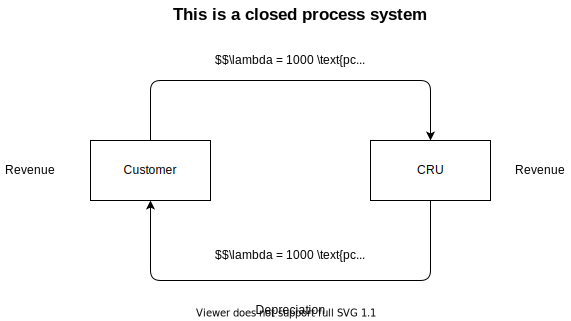
\includegraphics{assets/drawio/CRU.drawio.svg}
\caption{CRU}
\end{figure}

\begin{quote}
Utilization (as used in this case) = Inventory on rent \(\div\) Total
inventory owned by CRU \textbf{But utilization is an inadequate
performance measure}
\end{quote}

\hypertarget{process-flow-diagram}{%
\subsection{Process Flow Diagram}\label{process-flow-diagram}}

\begin{figure}
\centering
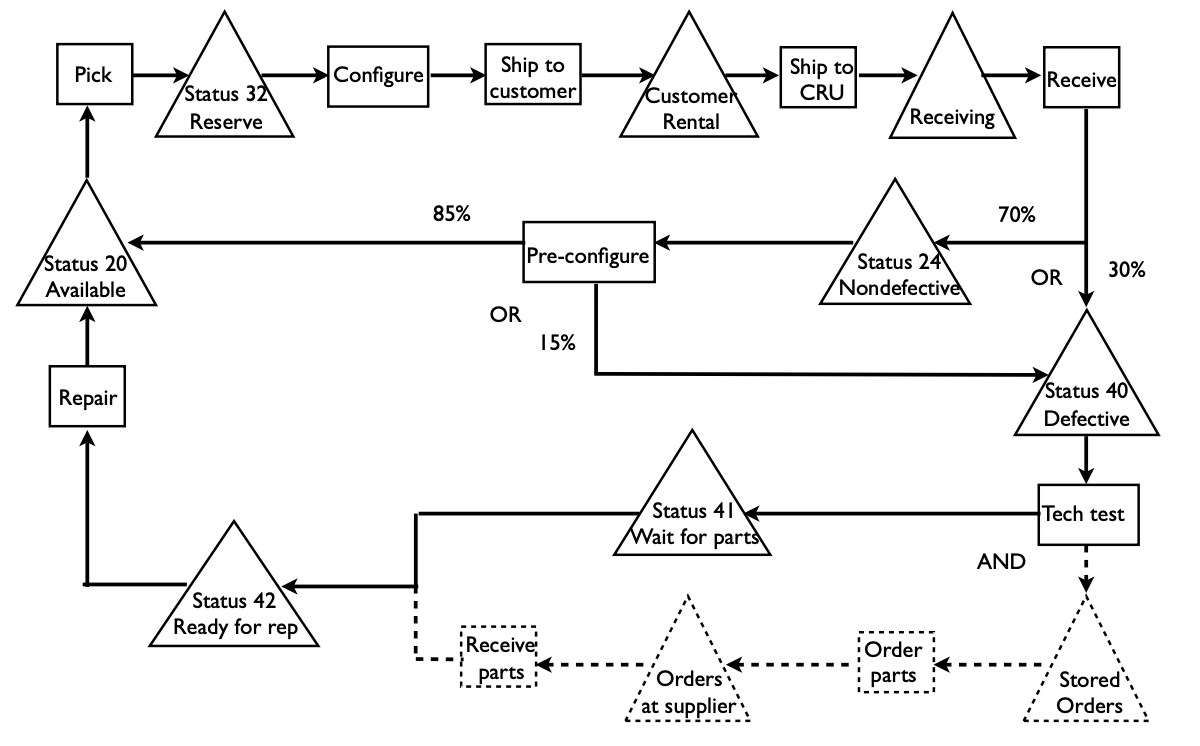
\includegraphics{assets/images/process-flow-CRU.png}
\caption{Process flow diagram}
\end{figure}

\textbf{Assumption}: Ignore WIP inventory at activities

\hypertarget{process-analysis}{%
\subsection{Process Analysis}\label{process-analysis}}

\begin{longtable}[]{@{}
  >{\raggedright\arraybackslash}p{(\columnwidth - 18\tabcolsep) * \real{0.1165}}
  >{\raggedright\arraybackslash}p{(\columnwidth - 18\tabcolsep) * \real{0.0874}}
  >{\raggedright\arraybackslash}p{(\columnwidth - 18\tabcolsep) * \real{0.0874}}
  >{\raggedright\arraybackslash}p{(\columnwidth - 18\tabcolsep) * \real{0.0874}}
  >{\raggedright\arraybackslash}p{(\columnwidth - 18\tabcolsep) * \real{0.0874}}
  >{\raggedright\arraybackslash}p{(\columnwidth - 18\tabcolsep) * \real{0.1262}}
  >{\raggedright\arraybackslash}p{(\columnwidth - 18\tabcolsep) * \real{0.1456}}
  >{\raggedright\arraybackslash}p{(\columnwidth - 18\tabcolsep) * \real{0.0874}}
  >{\raggedright\arraybackslash}p{(\columnwidth - 18\tabcolsep) * \real{0.0874}}
  >{\raggedright\arraybackslash}p{(\columnwidth - 18\tabcolsep) * \real{0.0874}}@{}}
\toprule
\begin{minipage}[b]{\linewidth}\raggedright
Metric
\end{minipage} & \begin{minipage}[b]{\linewidth}\raggedright
Customers
\end{minipage} & \begin{minipage}[b]{\linewidth}\raggedright
Receiving
\end{minipage} & \begin{minipage}[b]{\linewidth}\raggedright
Status 24
\end{minipage} & \begin{minipage}[b]{\linewidth}\raggedright
Status 40
\end{minipage} & \begin{minipage}[b]{\linewidth}\raggedright
Stored Orders
\end{minipage} & \begin{minipage}[b]{\linewidth}\raggedright
Supplier Orders
\end{minipage} & \begin{minipage}[b]{\linewidth}\raggedright
Status 41
\end{minipage} & \begin{minipage}[b]{\linewidth}\raggedright
Status 42
\end{minipage} & \begin{minipage}[b]{\linewidth}\raggedright
Status 20
\end{minipage} \\
\midrule
\endhead
\(\lambda\) & 1000 & 1000 & 700 & 405 & 405 & 405 & 405 & 405 & 1000 \\
\(\text{INV}\) & 8000 & 500 & 1500 & 1000 & 500 & 405 & 905 & 500 &
2000 \\
\(\text{CT}\) & 8 & 0.5 & 2.14 & 2.47 & 1.23 & 1 & 2.23 & 1.23 & 2 \\
\bottomrule
\end{longtable}

\end{document}